% Generated using docx2tex
%
% Compile with
% pdflatex -shell-escape DTS_Endpoint_v2_Firmware_Interface.tex
%
% Converted from https://docs.google.com/document/d/1ZzANOtcAxRvrJcFqc5HzPNJcnqltBSxY0-tVWq_L9B4/edit?usp=sharing
%
% docx2tex 1.7.3 --- ``Just out of this Word.'' 
% https://github.com/transpect/docx2tex 
%  
\documentclass{article} 
\usepackage[T1]{fontenc} 
\usepackage[utf8]{inputenc} 
\usepackage{graphicx}
\usepackage{hyperref} 
\usepackage{multirow} 
\usepackage{tabularx} 
\usepackage{color} 
\usepackage{textcomp} 
\usepackage{amsmath} 
\usepackage{amssymb} 
\usepackage{amsfonts} 
\usepackage{amsxtra} 
\usepackage{mathtools} 
\usepackage{enumerate} 
\usepackage{ulem} 
\usepackage[english]{babel}
\usepackage{minted}

\begin{document}
\title{DUNE Timing System (DTS) Endpoint v2 Interface}

\author{DMN}
\date{2022-02-23\\\normalsize Document version v3}

\maketitle
\newpage
\section{VHDL Declaration of Endpoint Interface}
\begin{minted}{vhdl}
  use work.pdts_ep_defs.all;

entity pdts_endpoint is
    generic(
        SCLK_FREQ: real;
        WAIT_HOST: boolean := false;
        USE_EXT_PLL: boolean := false;
        EXT_PLL_DIV: positive := 1;
        FORCE_TX: boolean := false;
        SKIP_FREQ: boolean := false;
        SKIP_ADDR: boolean := false;
        SKIP_DESKEW: boolean := false;
        SKIP_TSTAMP: boolean := false;
    );
    port(
        sys_clk: in std_logic;
        sys_rst: in std_logic;
        sys_addr: std_logic_vector(15 downto 0) := X"FFF0";
        sys_ctrl_in: in pdts_cmo := PDTS_CMO_NULL;
        sys_ctrl_out: out pdts_cmi;
        stat: out std_logic_vector(3 downto 0);
    ctrl_out: out pdts_cmo;
        ctrl_in: in pdts_cmi := PDTS_CMI_NULL;
        pll_clko: out std_logic;
        pll_clki: in std_logic := '0';
        los: in std_logic := '0';
        rxd: in std_logic;
        txd: out std_logic;
        txenb: out std_logic;
        clk: out std_logic;
        rst: out std_logic;
        ready: out std_logic;
        tstamp: out std_logic_vector(63 downto 0);
        sync: out std_logic_vector(3 downto 0);
        sync_stb: out std_logic
    );


\end{minted}

\section{Block Diagram of Endpoint and Host Firmware}

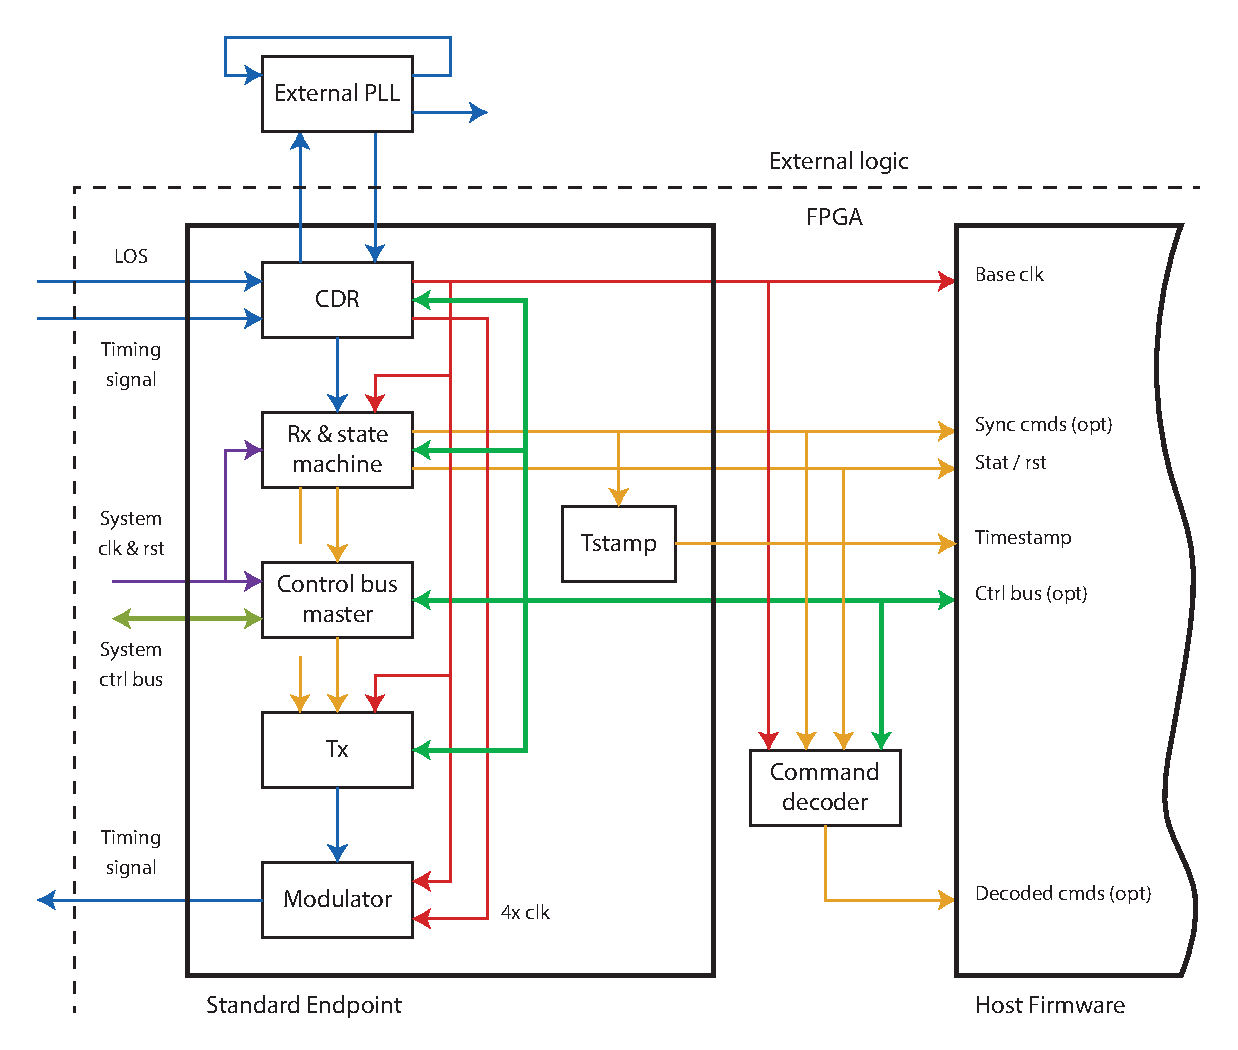
\includegraphics[width=1\textwidth]{endpoint_structure.pdf}


\section{General Notes}

The DTS endpoint is a common firmware block to be used by all DUNE readout systems connected to the timing system. It provides the following functionality:
\begin{itemize}
\item Recovery of the DUNE 62.5MHz clock and DTS packet data from the timing signal
\item Deskewing of clock and timing signals to \textasciitilde{}ns precision across all readout systems
\item Generation of the common DUNE 64b timestamp
\item Reception and decoding of timing alignment and command signals
\item Transmission of status and alignment information back to the timing master
\item Provision of status and debugging information to the host firmware
\item Read-write ‘out of band’ access to registers in the host firmware
\end{itemize}
The DTS is implemented in VHDL, and can be integrated into host firmware as source files or as a packaged IP block. In the former case, the VHDL package \texttt{pdts\_ep\_defs.vhd} provides the definitions of the necessary types and constants for the interface.

The DTS code is validated for Xilinx 7-series, Ultrascale and Ultrascale+ architectures. This document should be read alongside the ‘timing endpoint integration guide’, which gives tips on use and debugging.

\section{Endpoint Interface Signals}

The names in parenthesis indicate the direction and clock domain of each signal. \uline{Underlining} indicates that this is a signal mandatory for system operation. All signals are active high / rising edge unless stated otherwise.

\textbf{\uline{sys\_clk}} (in): Free-running system clock input from host firmware to endpoint. This clock needs to be in the range 10-100MHz, and be available continually during system operation.

\textbf{\uline{sys\_rst}} (in, sys\_clk): Synchronous reset signal from host firmware to endpoint. This must be asserted at any sys\_clk is not stable, and at system startup. Assertion of this signal during operation will cause an endpoint reset; this may also be triggered via the control bus.

\textbf{sys\_addr} (in, sys\_clk): Sets the address of the endpoint; can be overridden by a register setting via the control bus. Note that every endpoint in the DUNE system must have a unique address.

\textbf{sys\_ctrl\_in} (in, sys\_clk): Control bus signals from host firmware. The control bus signals and protocol are explained below.

\textbf{sys\_ctrl\_out} (out, sys\_clk): Host firmware control bus output.

\textbf{stat} (out, sys\_clk): System status word. This information is also available via the control bus. The endpoint startup sequence is detailed below. The possible states documented below.

\textbf{ctrl\_out} (out, clk): Slave control bus output to external logic (e.g. command decoder).

\textbf{ctrl\_in} (in, clk): Slave control bus input from external logic.

\textbf{pll\_clko} (out): 31.25MHz output clock to an external jitter-cleaning PLL, where this is used. This signal must be connected directly to a top-level output pin with no intervening logic, or left open if no external PLL is used.

\textbf{pll\_clki} (in): 62.5MHz input clock from an external jitter-cleaning PLL, where this is used. This signal must be connected directly to a top-level input pin with no intervening logic or buffers, or left open if no external PLL is used.

\textbf{los} (in): Loss-of-signal indicator from components in the external timing signal input path. Typically, this will be driven by the LOS pin of the timing SFP. This signal must be low for endpoint startup to complete, but can be left open if no LOS indicator is available.

\textbf{\uline{rxd}} (in): Timing signal input from optical receiver. This signal must be connected directly to a top-level output pin with no intervening logic.

\textbf{\uline{txd}} (out, clk): Timing signal output to optical transmitter. This signal must be connected directly to a top-level output pin with no intervening logic.

\textbf{\uline{txenb}} (out, clk, active-low): Timing signal output enable (active-low). This signal typically drives the TXDIS pin of the timing SFP.

\textbf{\uline{clk}} (out): 62.5MHz clock to the host firmware. This clock is available and stable after timing endpoint alignment, and may be unstable or absent during endpoint startup.

\textbf{\uline{rst}} (out, clk): Synchronous reset signal to host firmware. This is asserted until \textbf{clk} is available and stable, and can be used as a master reset for logic driven by the DUNE clock.

\textbf{\uline{ready}} (out, clk): Status indicator to host firmware. This is asserted when the endpoint internal state is ST\_READY and indicates that the various output signals from the endpoint are valid.

\textbf{\uline{tstamp}} (out, clk): Timestamp output to host firmware.

\textbf{sync} (out, clk): Timing command output to external decoder and / or host firmware. The meaning of individual timing commands is defined as part of the overall DUNE partitioning scheme.

\textbf{sync\_stb} (out, clk): TIming command strobe, asserted for one cycle when \textbf{sync} is valid.

\section{Endpoint Generics}

\textbf{SCLK\_FREQ}: Frequency of system clock \textbf{sys\_clk} in MHz.

\textbf{USE\_EXT\_PLL}: Causes the external PLL to be included in the clock decoder loop. The external PLL can be used for jitter reduction and / or propagation of the DUNE clock to hardware outside the FPGA.

\textbf{EXT\_PLL\_DIV}: Specifies the frequency of pll\_clki. EXT\_PLL\_DIV = 1 indicates that a 62.5MHz clock is returned, EXT\_PLL\_DIV = 2 specifies a 31.25MHz clock.

\textbf{FORCE\_TX}: Causes \textbf{txenb} to be permanently asserted, for testing purposes.

\textbf{SKIP\_FREQ}: Causes the frequency check step (see below) to be skipped; useful for simulation.

\textbf{SKIP\_ADDR}: Prevents the endpoint waiting for register settings for address; useful for simulation or testing, or where the address is permanently fixed via the \textbf{sys\_addr} port.

\textbf{SKIP\_DESKEW}: Prevents the endpoint waiting for register settings for deskew; useful for simulation or testing.

\textbf{SKIP\_TSTAMP}: Causes the timestamp alignment step (see below) to be skipped; useful for simulation or testing.

\section{Endpoint Startup}

The endpoint state machine proceeds through the following states:

\textbf{ST\_RESET} (0x0): Held in reset by an asserted \textbf{sys\_rst} signal.

\textbf{ST\_W\_SIG} (0x1): Waiting for \textbf{los} to be deasserted.

\textbf{ST\_W\_CLK} (0x2): Waiting for the (optional) external and internal PLLs to lock. \textbf{rst} is deasserted after this step.

\textbf{ST\_W\_FREQ} (0x3): Conducting a measurement of the frequency of the recovered clock; the clock frequency must be within \textasciitilde{}3000ppm of the nominal value to pass this step. This typically takes \textasciitilde{}1ms in real time, and can optionally be skipped.

\textbf{ST\_W\_CDR} (0x4): Waiting for the data recovery block to lock. This typically takes \textasciitilde{}8ms in real time.

\textbf{ST\_W\_RX} (0x5): Waiting for comma alignment.

\textbf{ST\_W\_SETUP} (0x6): Waiting for register settings (for address and deskew). This can optionally be skipped.

\textbf{ST\_W\_TS} (0x7): Waiting to receive a timestamp broadcast from the timing master. This can take up to \textasciitilde{}1s in real time, and can optionally be skipped.

\textbf{ST\_READY} (0x8): Fully operational; \textbf{ready} is asserted.

\textbf{ST\_ERR\_P} (0xc): An error in the physical layer (loss of signal, loss of lock, frequency drift) has been detected.

\textbf{ST\_ERR\_R} (0xd): An alignment or protocol error in the receiver has been detected. \textbf{rdy} is deasserted.

\textbf{ST\_ERR\_T} (0xe): Mis-alignment of the local and system timestamp has been detected.

In any of the error states, \textbf{ready} is deasserted and \textbf{rst} may be asserted if clock lock is lost. These states persist until the endpoint is reset via assertion of \textbf{sys\_rst} or via the control bus.

\section{Command Decoder Block}

The command decoder offers optional additional functionality for host firmware that needs to receive trigger, calibration or alignment commands via the timing system. The decoder recognises up to eight of the available 256 timing commands, and asserts one of eight one-hot decoded outputs when one of these eight is received. The mapping of timing commands to outputs is configurable either by the local system or by the timing master.

This allows the host system to flexibly use any combination of broadcast commands and commands directed to specific groups of hardware. The meaning of specific commands is not fixed, except in three cases:
\begin{itemize}
\item 0x0: \textbf{ts\_sync}, used internally within the timing system for timestamp broadcast. This signal is asserted exactly once per second, and can be used by the user firmware for other purposes if needed (e.g. alignment of ADC divided clocks between boards).
\item 0x1: \textbf{echo}, used internally within the timing system for timing delay calibration.
\item 0xff: \textbf{reserved\_0xff}, is never sent and should not be used by user firmware.
\end{itemize}
The host firmware may also decode the timing commands internally if required, noting that timing commands are not valid until \textbf{ready} is asserted.

\subsection{VHDL Entity Declaration of Decoder Interface}

\begin{minted}{vhdl}
entity pdts_ep_decoder is
    port(
        clk: in std_logic;
        rst: in std_logic;
        ctrl_in: in pdts_cmo;
        ctrl_out: out pdts_cmi;
        sync: in std_logic_vector(7 downto 0);
        sync_stb: in std_logic;
        cmd: out std_logic_vector(7 downto 0)
    );

end pdts_ep_decoder;
\end{minted}


\section{Control bus}

The system control bus allows access to the endpoint internal
registers, and to the registers of any blocks connected via the slave
control bus (e.g. the timing command decoder block or any other block
attached in the host firmware). These registers are accessible to the
host logic. The timing master can also access these registers via
control packets sent via the timing system. Access is arbitrated
between the system control bus and the timing master on a
transaction-by-transaction basis, with the timing master taking
precedence.

Note that the internal control bus runs on the 62.5MHz clock, with a
clock-domain crossing on between the system and base clock for the
system control bus interface. Registers are therefore NOT accessible
to the system controller until the base clock is stable; that is,
after the endpoint has reached at least the state
\textbf{ST\_W\_FREQ}. The user system controller should therefore
always monitor the \textbf{stat} status signal, which is available
regardless of the endpoint state.

The control bus signals are defined in \texttt{pdts\_ep\_defs.vhd} as follows:

\begin{itemize}
\item Master-to-slave signals:
\begin{itemize}
\item \textbf{a} (7b): register address
\item \textbf{d} (8b): register write data
\item \textbf{rw}: write / read flag (1 = write, 0 = read)
\item \textbf{stb}: transaction strobe
\end{itemize}

\item Slave-to-master signals:
\begin{itemize}
\item \textbf{d} (8b): register read data
\item \textbf{ack}: acknowledge flag
\end{itemize}

\end{itemize}

A simple two-stage handshake is used between master and slave:

\begin{itemize}
\item The master asserts \textbf{a}, \textbf{rw}, \textbf{stb} and \textbf{d} on a write transaction, and holds these signals at a constant value.
\item The slave carries out the commanded operation and asserts \textbf{ack}, along with \textbf{d} on a read transaction.
\item The master may begin another transaction on the cycle following the assertion of ack.
\end{itemize}

\textbf{stb} must be asserted until \textbf{ack} is asserted, and de-asserted on the cycle following this unless a new transaction is begun. Slaves are allowed to permanently assert \textbf{ack} if it is guaranteed that all read and write operations are completed in a single cycle. Address decoding and slave return data mutiplexing is the responsibility of the host firmware if the control bus is used. A timing diagram is shown below, illustrating four successive transactions: (a) a read cycle with wait states, (b) a write cycle with no wait state, (c) a read cycle with no wait state, (d) a write cycle with wait states. This bus operates in a similar fashion to IPbus or Wishbone, but with narrower address and data busses.


%\section{Timing diagrams}

\begin{figure}[p]
  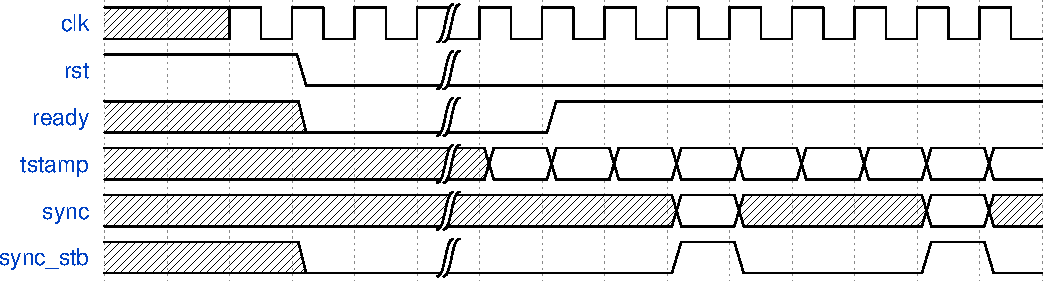
\includegraphics[width=1\textwidth]{dts_endpoint_startup_timing.pdf}% Generated from JSON file with Wavedrom
  \caption{Endpoint startup timing}
  \label{fig:endpoint_startup_timing}
\end{figure}

\begin{figure}[p]
  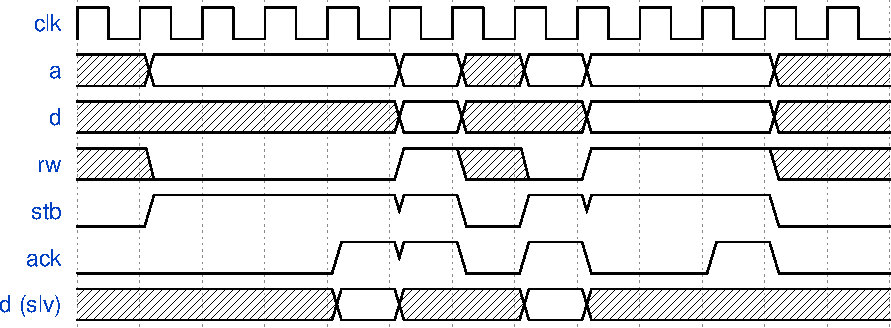
\includegraphics[width=1\textwidth]{dts_endpoint_ctrl_bus_timing.pdf}% Generated from JSON file with Wavedrom
  \caption{Endpoint control bus timing}
  \label{fig:endpoint_bus_timing}
\end{figure}


%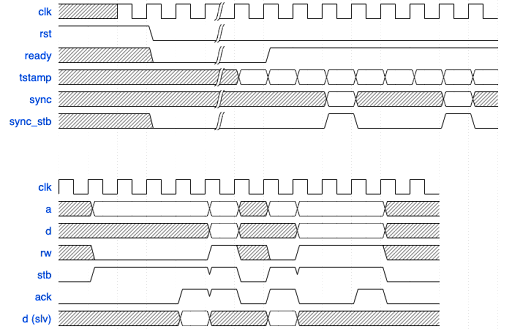
\includegraphics[width=1\textwidth]{dts_endpoint_timing_diagram.png}


\section{Register map}

\begin{table}[h!]
%\begin{tabularx}{\textwidth}{|l|l|l|l|l|} \hline 
\begin{tabularx}{\textwidth}{|
p{\dimexpr 0.096\linewidth-2\tabcolsep-2\arrayrulewidth}|
p{\dimexpr 0.239\linewidth-2\tabcolsep-\arrayrulewidth}|
p{\dimexpr 0.141\linewidth-2\tabcolsep-\arrayrulewidth}|
p{\dimexpr 0.08\linewidth-2\tabcolsep-\arrayrulewidth}|
p{\dimexpr 0.443\linewidth-2\tabcolsep-\arrayrulewidth}|} \hline
\textbf{Addr} & \textbf{Decoding block} & \textbf{Name} & \textbf{RW} & \textbf{Content} \\\hline 
0x00 - 0x5f   & User firmware           &               &               & User registers \\\hline 
0x60          & \multirow{8}{=}{Command decoder}  & tcmd\_0 & rw & \multirow{8}{=}{Trigger decoder commands \#0 - \#7}  \\\cline{1-1}\cline{3-4}
0x61          &                         & tcmd\_1 & rw &  \\\cline{1-1}\cline{3-4}
0x62          &                         & tcmd\_2 & rw &  \\\cline{1-1}\cline{3-4}
0x63          &                         & tcmd\_3 & rw &  \\\cline{1-1}\cline{3-4}
0x64          &                         & tcmd\_4 & rw &  \\\cline{1-1}\cline{3-4}
0x65          &                         & tcmd\_5 & rw &  \\\cline{1-1}\cline{3-4}
0x66          &                         & tcmd\_6 & rw &  \\\cline{1-1}\cline{3-4}
0x67          &                         & tcmd\_7 & rw &  \\\hline 
0x68 - 0x6f   & Timestamp               & tstamp & rw & Timestamp set / check value \\\hline 
0x70          & \multirow{6}{=}{Endpoint}  & ctrl & rw & b0 rx reset (restarts lock process, does not clear registers) \newline b1 address set flag \newline b2 deskew set flag \newline b3 update clock phase \newline b7 hard reset (clears registers) \\\cline{1-1}\cline{3-5}
0x71          &        & stat & ro & b3:0 endpoint status word \newline b4 clock phase update complete \\\cline{1-1}\cline{3-5}
0x72 - 0x73   &        & deskew & rw & b3:0 coarse delay \newline b15:4 clock phase (i.e. fine delay) \\\cline{1-1}\cline{3-5}
0x74 - 0x75   &        & addr & rw & Endpoint address \\\cline{1-1}\cline{3-5}
0x76          &        & err\_cnt & rw & Count of soft protocol errors; write to register clears \\\cline{1-1}\cline{3-5}
0x77          &        & version & ro & Endpoint version \\\hline 
\end{tabularx}
  \caption{Endpoint control bus address map}
  \label{tab:endpoint_ctrl_bus_addr_map}
\end{table}

\end{document}
